%
% File coling2014.tex
%
% Contact: jwagner@computing.dcu.ie
%%
%% Based on the style files for ACL-2014, which were, in turn,
%% Based on the style files for ACL-2013, which were, in turn,
%% Based on the style files for ACL-2012, which were, in turn,
%% based on the style files for ACL-2011, which were, in turn, 
%% based on the style files for ACL-2010, which were, in turn, 
%% based on the style files for ACL-IJCNLP-2009, which were, in turn,
%% based on the style files for EACL-2009 and IJCNLP-2008...

%% Based on the style files for EACL 2006 by 
%%e.agirre@ehu.es or Sergi.Balari@uab.es
%% and that of ACL 08 by Joakim Nivre and Noah Smith

\documentclass[11pt]{article}
\usepackage{coling2014}
\usepackage{times}
\usepackage{url}
\usepackage{latexsym}
\usepackage{graphicx}

%\setlength\titlebox{5cm}

% You can expand the titlebox if you need extra space
% to show all the authors. Please do not make the titlebox
% smaller than 5cm (the original size); we will check this
% in the camera-ready version and ask you to change it back.


\title{An Analysis of Multiword Expressions in the Paraphrase Database}

\author{First Author \\
  Affiliation / Address line 1 \\
  Affiliation / Address line 2 \\
  Affiliation / Address line 3 \\
  {\tt email@domain} \\\And
  Second Author \\
  Affiliation / Address line 1 \\
  Affiliation / Address line 2 \\
  Affiliation / Address line 3 \\
  {\tt email@domain} \\}

\date{}

\begin{document}
\maketitle
\begin{abstract}
We investigate whether paraphrases might be a useful resource for understanding multiword expressions (MWEs).  In particular, we analyze the paraphrases in PPDB, the Paraphrase Database, where multiple words are re-written as a single word.  By automatically mapping from multiword expressions onto single words, NLP systems could potentially process the re-written text more easily than the original text containing MWEs. We use the MWE categorization system as described in \newcite{BaldwinCategorization}.  Although a small proportion of the many-to-one paraphrases in PPDB are classic MWEs, the resource contains millions of entries.  We therefore train a classifier to distinguish interesting MWEs from other sorts of many-to-one paraphrases.
\end{abstract}

\section{Introduction}
\label{intro}

%
% The following footnote without marker is needed for the camera-ready
% version of the paper.
% Comment out the instructions (first text) and uncomment the 8 lines
% under "final paper" for your variant of English.
% 
\blfootnote{
    %
    % for review submission
    %
    \hspace{-0.65cm}  % space normally used by the marker
    Place licence statement here for the camera-ready version, see
    Section~\ref{licence} of the instructions for preparing a
    manuscript.
    %
    % % final paper: en-uk version (to license, a licence)
    %
    % \hspace{-0.65cm}  % space normally used by the marker
    % This work is licensed under a Creative Commons 
    % Attribution 4.0 International Licence.
    % Page numbers and proceedings footer are added by
    % the organisers.
    % Licence details:
    % \url{http://creativecommons.org/licenses/by/4.0/}
    % 
    % % final paper: en-us version (to licence, a license)
    %
    % \hspace{-0.65cm}  % space normally used by the marker
    % This work is licenced under a Creative Commons 
    % Attribution 4.0 International License.
    % Page numbers and proceedings footer are added by
    % the organizers.
    % License details:
    % \url{http://creativecommons.org/licenses/by/4.0/}
}

Multiword expressions (MWEs) are phrases whose meanings are different than the literal interpretation of the words in the phrase. MWEs include verb-particle constructions, fixed expressions, compound nominals, and decomposable idioms, to name a few \cite{Sag2002}.  MWEs are difficult to process both for non-native speakers of English, as well as for NLP systems. Studies using an eye-movement paradigm have found that non-native speakers of English required more time to retrieve figurative senses of phrases than literal ones, whereas native speakers retrieved the idiomatic meaning faster than the literal meaning (Siyanova-Chanturia and Martinez, 2014). These studies imply that L2 speakers of English may find it more difficult to understand MWEs than a similar phrase whose meaning was literal.  Among NLP systems, both parsers and information retrieval systems make errors on MWEs. As described by \newcite{Villavicencio2007,Baldwin2004} found that, among a random sample of 20,000 strings from the written portion of the British National Corpus \citep{Burnard2000}, using the English Resource Grammar \citep{Copestake+Flickinger2000}, MWEs caused 8\% of all parse errors. When manually­ selected compound nominals were searched for as single terms it improved information retrieval results \citep{Acosta2011}.

Based on this information, it seems that identifying MWEs could be useful for NLP tasks. In this paper we use the Paraphrase Database (PPDB) as a resource to define a MWE lexicon, which could be incorporated into other NLP systems.

The Paraphrase Database (PPDB) is a database containing English paraphrases. PPDB was developed using alignment techniques from machine translation on bilingual parallel corpora, pivoting on a foreign language, to find English phrases that translate to the same foreign-language phrase (Bannard and Callison-Burch, 2005). The database takes into account syntactic information of both the English and foreign-language phrases: the entries in PPDB were found using SCFGs to come up with paraphrases that form constituents of the same syntactic category (Ganitkevich et al, 2011; Ganitkevich et al, 2013).

\section{Experimental Design}
The Paraphrases Database (PPDB) contains English paraphrases. We have characterized a subset of the paraphrases found in the PPDB, according to categories of multi-word expressions (MWEs), syntactic changes in the expansion from a word to its paraphrase, and what parts of speech appear in the corpus. We also looked at how many of the paraphrases in the PPDB appear to be spurious.

The categories of MWEs we looked at were light verbs, verb-particle constructions, negation, and superlatives. We also included Tim Baldwin's categories for MWEs: fixed expressions, non-decomposable idioms, compound nominals, proper names, and decomposable idioms. 

In addition to MWE categories, we also included categories for syntactic changes from a word to its paraphrase: change of tense followed by a paraphrase, nominalizations, infinitival to, adverbial modifier, one or more words the same as part of the original word, determiner followed by a one-word paraphrase, determiner followed by the plural form, and change of tense. Finally, we included acronyms, hypernym-hyponym pairs, times, extra punctuation marks, and numbers as categories, as well as unspecified expansions and bad paraphrases.

\section{Results}

Of a random sample of 500 paraphrases from the L one-to-many paraphrase file, the most common types of paraphrase were expansions using the same morphological form (117 instances, or 23.4\%), determiner followed by a one-word paraphrase (86 instances, or 17.2\%), and paraphrases that did not fall into a particular category (62 instances, or 12.4\%). Of the sample, 43 were bad paraphrases (8.6\%). The full list of categories and the number of instances in each are in the table below.  

Of the 500 paraphrases in the random sample, 37 (7.4\%) fell into the MWE categories defined by Baldwin et al. Of these MWE paraphrases, the most common were verb-particle constructions (14 instances, or 37.8\%) , followed by proper names (7, or 18.9\%). There were no instances of compound nominals in the sample.

The full list of categories with the number of instances of paraphrases in each, as well as illustrative examples for each, are in the table below (Table 1). MWEs, as defined by Baldwin et al., are marked in bold. 

\begin{table}[h]
\begin{center}
\begin{tabular}{|l|r|l|}
\hline \bf Paraphrase Category & \bf Number of & \bf Examples \\ 
 & \bf instances & \\
 & \bf in sample & \\ \hline
determiner + one-word paraphrase & 86 & photographs, the images; duties, the responsibilities \\
expansion & 62 & suffocate, need air; cumbersome, time consuming \\
expansion, same morphological form & 47 & fun, sounds like fun; signs, signs and signals \\
change of tense + paraphrase & 43 & initiated, has undertaken; say, going to tell \\
inaccurate/bad paraphrase & 43 & iron, a par; also, do i\\
implicit/most common modifier & 41 & baghdad, iraqi capital baghdad; \\
&& enrichment, uranium enrichment \\
implicit type & 29 & training, training course; customs, customs offices \\
adverbial modifier& 27 & interesting, very interesting; more, even more \\
acronym & 21 & gpa, the global programme of action; cras, \\
&& credit-rating agencies \\
one or more words  & 17 &  anytime, any point; enslavement, slave labour \\
the same as part of original word & &\\
\bf verb-particle & 14  & torched, burnt down; done, carried out\\
determiner + plural & 9 & gloves, the glove; militaries, the military\\
\bf proper noun & 7 & markov, mr markov; karadzic, radovan karadzic\\
change of tense & 7 & changing, be changed; attain, be attained\\
\bf fixed expression & 6 & applied, put into effect; plenty, a whole host \\
superlative & 5 & notably, most particularly; best-known, most famous\\
copula & 5 & qualify, are eligible; reason, been right \\
\bf decomposable idiom & 4 & nuts, out of your mind; sleeping, get a good night's sleep\\
\bf light verb & 4  &  issued, made available; place, make way \\
number & 4 & 20, twenty of; 5,000, 5 000\\
infinitival to & 3 & track, to follow; answer, to reply \\
nominalization & 3 &  operation, proper functioning \\
negation & 2 & unused, not utilized; non-parties, not parties  \\
time variation & 2 & 7:00, seven hours; 2003/04, the 2003-04 fiscal year\\
punctuation & 2 & debt-servicing, debt servicing; what, somethin '\\
\bf non-decomposable idiom & 2 & furious, as mad as hell; entails, brings with it\\
alternate spelling & 1 & al-najaf, al nagaf\\
\bf compound nominal & 0 &\\
\hline
\end{tabular}
\end{center}
\caption{\label{font-table} Number of instances from each category in random sample of 500. }
\end{table}

The distribution of the parts of speech from this random sample is depicted in the histogram below. 

\begin{center}
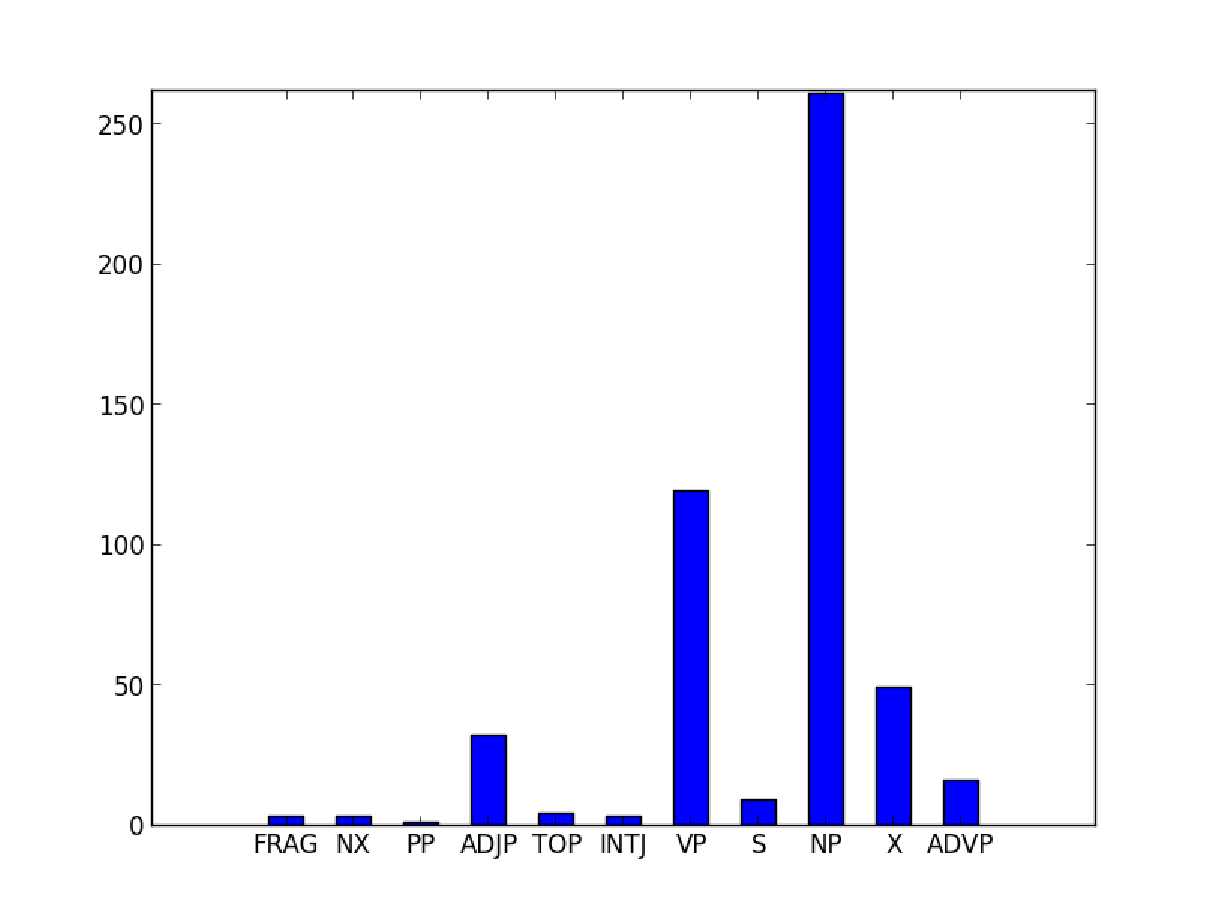
\includegraphics[width=150mm]{figs/random_sample_pos_histogram_500.pdf}
\end{center}

The distribution of all of the parts of the speech from the L one-to-many paraphrase file is depicted in the following histogram:

\begin{center}
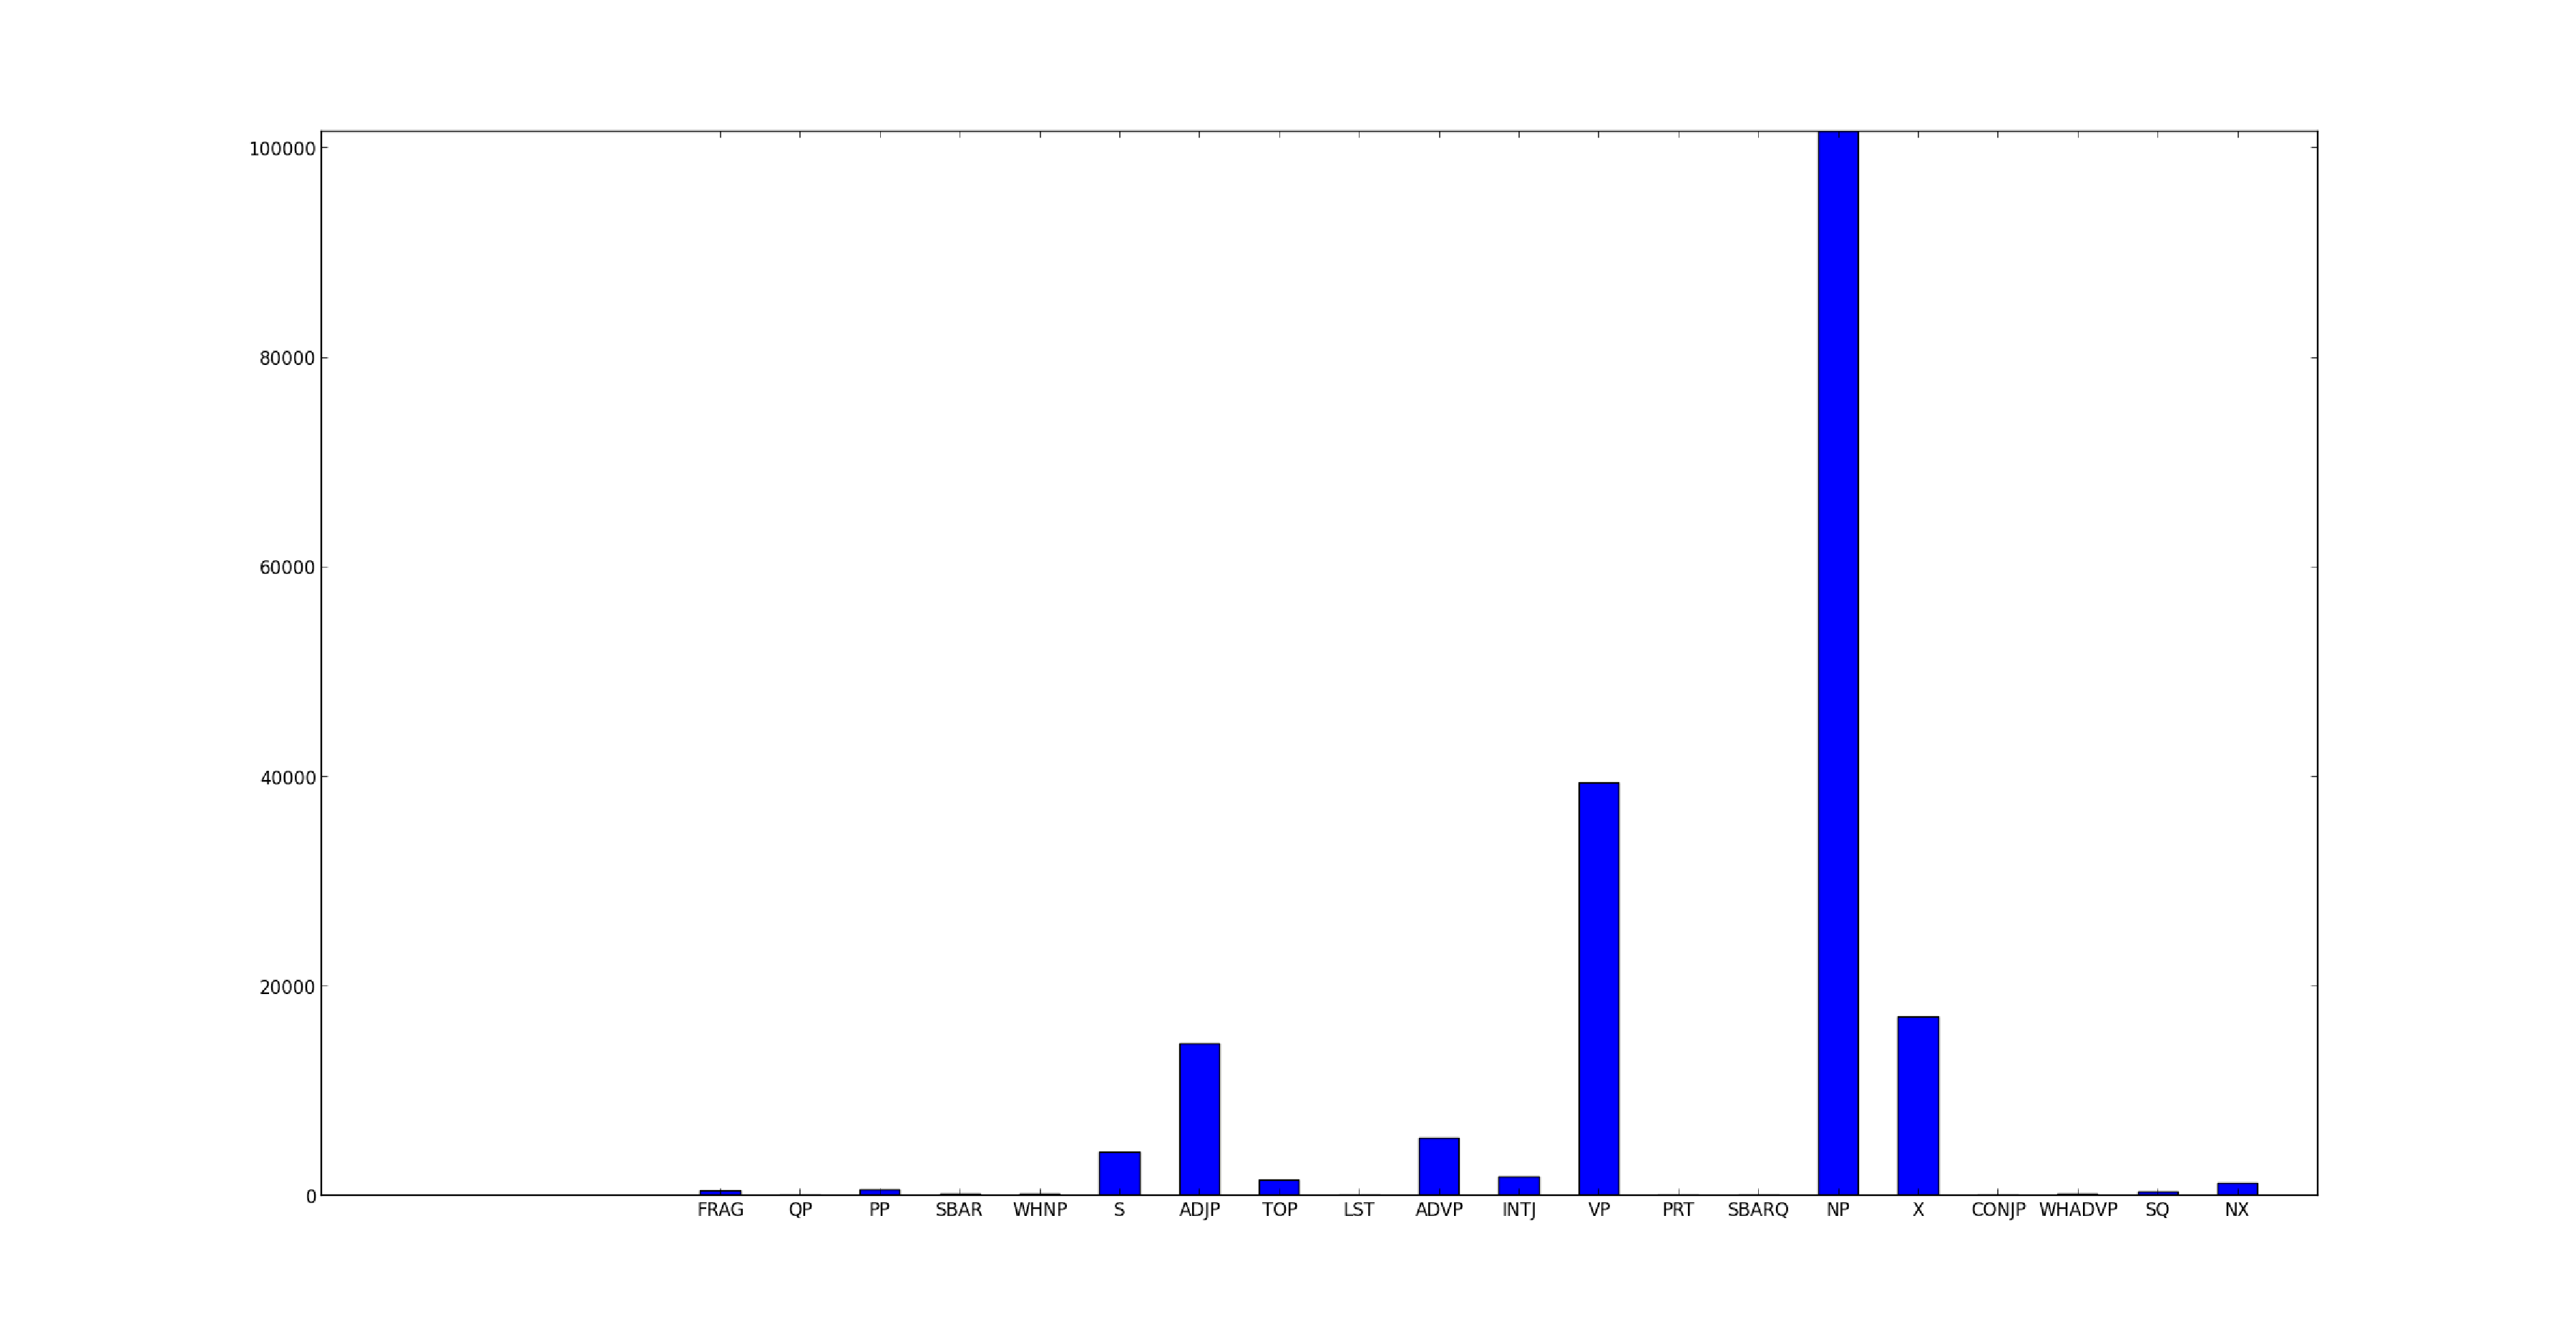
\includegraphics[width=175mm]{figs/random_sample_pos_histogram_all.pdf}
\end{center}

In both samples, the most common part of speech is NP, followed by VP. 


In addition to categorizing a random sample of paraphrases, we searched for instances of light verbs, verb-particle constructions, negation, comparatives, and superlatives. The light verbs were those with the verb “have”, “take”, “make”, “hold” or “give, ” followed by a noun phrase. The verb-particle constructions were any verbs followed by the particles “down”, “up”, “on”, “out”, “over” or “upon.” Negation instances had the word “not” either in the original or the expanded paraphrase. Comparatives had the word “more,” and superlatives had the word “most.”

To find instances of verb-particle constructions, we used the Linux command 'grep' and the regular expression ' particle\b' to find phrases where the potential particle was not the first word, and to ensure that it was not a substring of another word (e.g., 'onto' instead of 'on'). For example, to find potential instances of verb-particle constructions with the particle 'up', we ran the following command:
grep ' up\b' ppdb-1.0-l-o2m

We then determined manually whether the phrases found were verb-particle constructions. The potential particle was sometimes a preposition or adverb, in which case it did not fit into this MWE category. 

We used similar commands to find instances of the other paraphrase categories. A list of the commands used is in the following table:

\begin{table}[h]
\begin{center}
\begin{tabular}{|l|rl|}
\hline \bf Paraphrase category & \bf Search command & \\ \hline
verb-particle construction & grep ' up \textbackslash b' ppdb\textunderscore filename &\\
light verbs & grep '\textbackslash b make ' ppdb\textunderscore filename &\\
negation & grep '\textbackslash b not ' ppdb\textunderscore filename &\\
comparatives & grep '\textbackslash b more ' ppdb\textunderscore filename &\\
superlatives & grep '\textbackslash b most ' ppdb\textunderscore filename &\\
\hline
\end{tabular}
\end{center}
\caption{\label{font-table} Linux commands to search for paraphrases of different types. }
\end{table}

The results from these searches are summarized in the tables below. We considered only light verb phrases with no extra terms (e.g., 'have a word', but not 'have a word with you' or 'can i have a word').

\begin{table}[h]
\begin{center}
\begin{tabular}{|l|r|l|}
\hline \bf Light verb & \bf Number of light verb phrases & \bf Number of light verb phrases\\ 
 & & \bf  found by grep \\ \hline
make & 35 & 46 \\
have & 45 & 105 \\
give & 4 & 11 \\
take & 33 & 48 \\
hold & 1 & 3 \\
\hline
\end{tabular}
\end{center}
\caption{\label{font-table} Light verbs. }
\end{table}


\begin{table}[h]
\begin{center}
\begin{tabular}{|l|r|l|}
\hline \bf Particle & \bf Number of verb-particle  & \bf Number of verb-particle\\ 
 & \bf constructions found & \bf  phrases found by grep \\ \hline
up & 439 & 439 \\
about & 10 & 115 \\
around & 44 & 47 \\
back & 145 & 156 \\
down & 190 & 195 \\
in & 32 & 207 \\
off & 134 & 134 \\
on & 109 & 196 \\
out & 383 & 383 \\
over & 65 & 67 \\
\hline
\end{tabular}
\end{center}
\caption{\label{font-table} Verb-particle constructions. }
\end{table}

After manually identifying categories, we developed a classifier to automatically find paraphrases that are interesting to MWE researchers. We built the classifier to find the following categories of MWE: verb-particle construction; expansion, same morphological form; implicit/most common modifier; implicit type; light verb; fixed expression; non-decomposable idiom; proper noun; decomposable idiom; light verb. 

The features we used were whether a preposition appeared in the expansion of the paraphrase (feature value either 1 or 0), whether the original word appeared in the expansion, whether a light verb appeared in the expansion, and all of the scores from the PPDB (every number that appeared in the entry following an equal sign).

The prepositions and light verbs used for the features are listed in the table below.

\begin{table}[h]
\begin{center}
\begin{tabular}{|l|rl|}
\hline \bf prepositions &  'about', 'around', 'back', 'down', 'in', 'off', 'on', 'out', 'over', 'up'  &\\ \hline
\bf light verbs &  'give', 'have', 'hold', 'make', 'take' &\\
\hline
\end{tabular}
\end{center}
\caption{\label{font-table} Words used as features for classifier. }
\end{table}

We used an SVM classifier (libsvm) with these features on our sample of 500 words. With ten-fold cross-validation, the accuracy of the classifier was 75.4%. By comparison, a baseline classifier that returns the majority class has an accuracy of 69.2%. 

%
% We are not doing the following for Coling 2014. Maybe next time.
%
% \section{XML conversion and supported \LaTeX\ packages}
% 
% ACL 2014 innovates over earlier years in that we will attempt to
% automatically convert your \LaTeX\ source files to machine-readable
% XML with semantic markup. This will facilitate future research that
% uses the ACL proceedings themselves as a corpus.
% 
% We encourage you to submit a ZIP file of your \LaTeX\ sources along
% with the camera-ready version of your paper. We will then convert them
% to XML automatically, using the LaTeXML tool
% (\url{http://dlmf.nist.gov/LaTeXML}). LaTeXML has \emph{bindings} for
% a number of \LaTeX\ packages, including the ACL 2014 stylefile. These
% bindings allow LaTeXML to render the commands from these packages
% correctly in XML. For best results, we encourage you to use the
% packages that are officially supported by LaTeXML, listed at
% \url{http://dlmf.nist.gov/LaTeXML/manual/included.bindings}


\section{Analysis}


%\section*{Acknowledgements} 
%This material is based on research sponsored by the NSF under grant IIS-1249516 and DARPA under agreement number FA8750-13-2-0017 (the DEFT program). The U.S. Government is authorized to reproduce and distribute reprints for Governmental purposes. The views and conclusions contained in this publication are those of the authors and should not be interpreted as representing official policies or endorsements of DARPA or the U.S. Government.

% include your own bib file like this:
%\bibliographystyle{acl}
%\bibliography{acl2014}


\end{document}
